% Définition du nom du chapitre
\chapter{Monitoring of } \label{chapitre5-capferrat}

%%%%%%%%%%%%%%%%%%%%%%%%%%%%%
%%% Figure cover chapitre %%%
%%%%%%%%%%%%%%%%%%%%%%%%%%%%%
\pagestyle{main}
\begin{figure}[H] 
	\begin{center}
	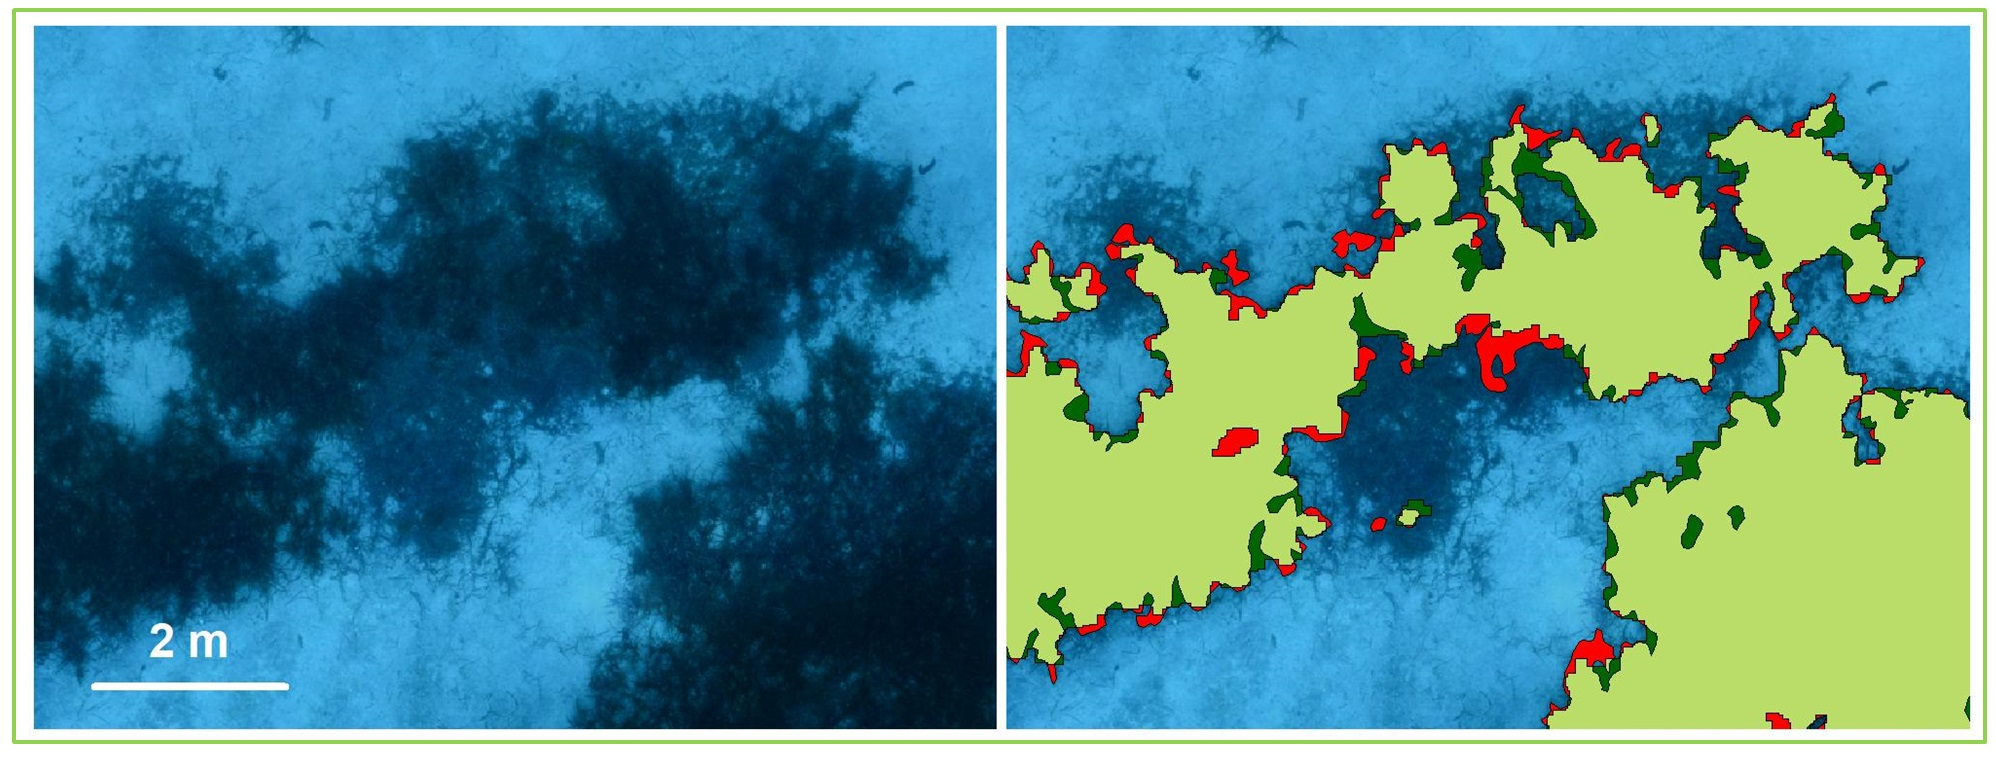
\includegraphics[width=\linewidth]{./chapitre5/cover.jpg}
    \end{center}
\end{figure}

% Bullet points du début de chapitre
\begin{colbox}{resume}
  \vspace{-2pt}
{\color{textresume}\small
\begin{itemize}[leftmargin=0in]\itemsep3pt
\item les garrigues sont des milieux naturels méditerranéens ouverts, caractérisés par une végétation très hétérogène~;
\item cette hétérogénéité se caractérise par l'assemblage en mosaïque de quatre strates verticales à une échelle très fine~: le sol nu, l'herbe, les ligneux bas et les ligneux hauts~;
\item l'hétérogénéité de cette mosaïque varie de manière continue dans le paysage~;
\item cette hétérogénéité est associée à une très forte biodiversité floristique et faunistique~;
\item cette hétérogénéité est la résultante~:
\begin{itemize}
  \item d'une importante variabilité climatique et topographique~;
  \item d'activités humaines qui ont façonné les milieux de garrigues~;
\end{itemize}
\end{itemize}
}
\vspace{-2pt}
%\end{fullminipage}
\end{colbox}

\clearpage

\noindent\textbf{Fine scale monitoring of living Posidonia oceanica}

% Auteurs
\noindent Guilhem Marre, Florian Holon, Sandra Luque, Pierre Boissery et Julie Deter

% NB sans indentation
\noindent\textit{En cours de révision dans...}

\noindent\textbf{Abstract}


\noindent\textbf{Keywords}


\section{Introduction}\label{chapitre5_1}

\section{Materials and methods}\label{chapitre5_2}

\section{Results}\label{chapitre5_3}

\section{Discussion}\label{chapitre5_4}

\section{Conclusion}\label{chapitre5_5}

\section{Conflict of interest}\label{chapitre5_6}
The authors declare that the research was conducted in the absence of any commercial or financial relationships that could be construed as a potential conflict of interest.

\section{Author contributions}\label{chapitre5_7}


\section{Funding}\label{chapitre5_8}
This study beneficiated from a financing of the French Water Agency (\acrlong{aermc}) (convention n° 2017-1118) and the LabCom InToSea (ANR Labcom 2, Université de Montpellier UMR 9190 MARBEC / Andromède Océanologie). Guilhem Marre received a PhD grant (2017-2020) funded by Agence Nationale pour la Recherche Technologique (ANRT) and Andromède Océanologie.

\section{Acknowledgments}\label{chapitre5_9}
